\documentclass{bmvc2k}

%% Enter your paper number here for the review copy
\bmvcreviewcopy{134}

\title{ Skeleton-Based Action Recognition\\ Using Few Shot Learning}
\usepackage{amsfonts}
\usepackage[ruled]{algorithm2e}
% Enter the paper's authors in order
% \addauthor{Name}{email/homepage}{INSTITUTION_CODE}
\addauthor{Wangbin Ding}{yomynan@gmail.com}{1}
\addauthor{Shengqin Lin}{http://www.vision.inst.ac.uk/~pp}{2}
\addauthor{Zhenze Dai}{b282078355@gmail.com}{2}

% Enter the institutions
% \addinstitution{Name\\Address}
\addinstitution{
 The Vision Institute\\
 University of Borsetshire\\
 Wimbleham, UK
}
\addinstitution{
 Collaborators, Inc.\\
 123 Park Avenue,\\
 New York, USA
}

\runninghead{Student, Prof, Collaborator}{Wangbin Ding}

\newcommand{\reffig}[1]{Figure \ref{#1}}
\newcommand{\reftab}[1]{Table \ref{#1}}


% Any macro definitions you would like to include
% These are not defined in the style file, because they don't begin
% with \bmva, so they might conflict with the user's own macros.
% The \bmvaOneDot macro adds a full stop unless there is one in the
% text already.
\def\eg{\emph{e.g}\bmvaOneDot}
\def\Eg{\emph{E.g}\bmvaOneDot}
\def\etal{\emph{et al}\bmvaOneDot}

%-------------------------------------------------------------------------
% Document starts here
\begin{document}

\maketitle

\begin{abstract}
This paper presents a new skeleton-based action recognition method using a few shot learning. Consider the sequence data contain the temporal and spatial information; the proposed method encodes each of skeleton as an RGB image. Nothing more but a naïve normalization is engaged to each channel of the encoded skeleton image. In order to acquire the discriminative skeleton image feature, a serial of dilated-dense layers is adopted in our model to both extend the receptive field of feature points and capture diversity representation of the skeleton image. After that, a prototypical network is introduced to recognize the specific action of the feature stands for. The skeleton image feature will be mapped into a metric space in which action classification can be performed by the nearest neighbor search. Benefited from the nature of the few shot learning, our model can be trained with only a few labeled samples. Moreover, it could deal with the samples from unseen classes that have not presented during the training phase. We evaluated our method with the seen and unseen class of samples, experiment result shows, the method achieved comparable performance on benchmark datasets even with a few support samples.

\textbf{Index Terms:}
skeleton sequence, dilated-dense layer, few shot learning
\end{abstract}

%-------------------------------------------------------------------------
\section{Introduction}
\label{sec:intro}
Human action recognition has been widely researched for a few decades. A lot of recognition methods are developed to serve for entertainment, surveillance, and video analysis. At present, the action recognition algorithm has made a great step forward by the wave of the deep learning model. However, these methods consume large-scale of training samples to capture the inner pattern of every action. As human action category is varied, the demand for training sample will explode. Besides, when new unseen actions are acceded to the classification task, the deep model need to be retrained to adapt the changing quantity of the action. A sort of few-shot (one-shot, zero-shot) learning methods are proposed to resolve these issues. Given a few of new action samples, these method can quickly accommodate the increasing new classes. Non-parameter model from nearest neighbor to metric learning [13] have played a significant role in the progress of this field. Mishra [14] present a generative framework for Zero-Shot or Few-Shot action recognition. Yang [15] introduce a new example-based action detection on the Matching Network. Nevertheless, seldom attention had been paid to apply the few shot learning model to skeleton sequence yet. To address this challenge, we propose an action recognition method based on the prototypical network. It can learns a metric space in which classification can be performed by computing distances to prototype representations of each class [19]. Because we had engaged a serial of CNN layers to extract the feature of skeleton sequence, our method also can benefit from the performance of CNN. And The main contributions of this method are:

1.	Only a few skeleton sequences are adequate to train an efficient action recognition model.

2.	With few support samples, it is enough to recognize the action that had never seen before.

3.	Dilated-dense layer is embedded to extract the feature maps, which can enhance the robustness and diversity of the feature representation. 

The remainder of the paper is organized as follows. In Sec.2 we briefly review methods proposed to deal with skeleton-based action recognition. In Sec.3 the representation of the skeleton using dilated-dense layer is introduced. Then the inference and training algorithm of our few shot learning based model will be fully described. In Sec.4 we report the experiments results on a series of datasets to show the performance of the method. Finally, in Sec.5 we discuss research directions in the future work.


\section{Related Work}
From the perspective of feature representation, skeleton-based action recognition methods can be divided into three main streams. 
The first streams usually encode the skeleton sequence into a skeleton-image. Different skeleton-image encoders are proposed to capture the feature of actions. Wang [1] introduce a compact and effective method to encode spatiotemporal information carried in 3D skeleton sequences into Joint Trajectory Maps (JTM). Pham[2] and Li[3] rearrange the pixels in RGB skeleton-images to obtain a better representation of the movement. Furthermore, Liu[4] design a skeleton visualization method to represent a skeleton sequence as a series of visual and motion enhanced color images. Having encoded skeleton sequences into skeleton images, a variety of CNN networks(CNN[1], multi-scale CNN[5], DeepResidualNeuralNetworks[2], multi-stream CNN[4]) are constructed to classify the indeed action of the skeleton image. 

The second steam is inspired by the RNN network, whose recurrent structure can boil a sequence data down into a high-level understanding []. For better performance, they tend to adopt the LSTM to process the skeleton sequence data. Zhu [6] introduce an end-to-end fully connected deep LSTM network with a designed regularization, through which can learn the co-occurrence feature of the skeleton joints. Based on LSTM, Liu [7] design a skeleton tree traversal method and a new gating mechanism to achieve a robust representation of the input sequence data. To further, Liu [8] also add attention ability to the LSTM network, which is capable of focusing on the informative joints of the skeleton.
The last one is based on graph convolutional network [9], which can be applied directly to the raw skeleton data. Shi [10] present a novel two-stream nonlocal graph convolutional network for the recognition task. Li [11] introduce multi-scale graphical convolutional kernels to encode motion variations and input state for feature extracting. Si [12] propose a novel Attention Enhanced Graph Convolutional LSTM Network, which can not only capture discriminative features in spatial configuration and temporal dynamics but also explore the co-occurrence relationship between spatial and temporal domains.

\section{Proposed Method}
\subsection*{Skeleton Image Encoder}
It is common knowledge that a skeleton sequence can be represented as an RGB image []. Consider an n frame action $a=\{ fr^1,fr^2,\cdots fr^n\}$, each frame $fr^i$ contains $m$ joints $fr^i =\{j^i_1,j^1_2,\cdots j^i_m\} $. And each joint $j^i_t=\{j^i_{tx},j^i_{ty},j^i_{tz}\}$ is a 3-D coordinate point, which is corresponding to the RGB channel of a pixel in a skeleton image. Thus, the skeleton sequence S can be encoded as an $m\times n$ skeleton image. a sort of variant RGB encoder had proposed to achieve the translation-scale invariant representation of the skeleton sequences [4 16,17]. But our method hasn’t taken advantage of these mechanisms. Only a naive normalization, proposed by [18], is adopted.

$$p'_k=floor(255*\frac{(p_k-p^{min}_k)}{\max \limits_{k}(p_k^{max}-p_k^{min})})$$

Where $p^{max}_k$ and $p^{min}_k$ are the maximum and minimum value of the k-th channel (x; y; z) of a skeleton. In this way, each action sample $a$ can be encoded into a skeleton image $I$.
\begin{figure}[htb] 
\centering
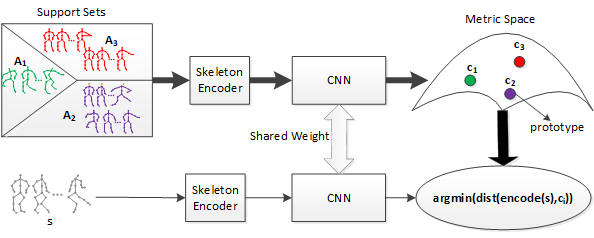
\includegraphics[height=1.8in]{images/Figure_1.png}
\caption{the workflow of extracting a skeleton image from a skeleton sequence}
\label{fig:1}	
\end{figure}

\subsection*{Dilated-Dense Layers}
\flushleft
The learnable part of our model is the mapping function $F_W:\mathbb{R}^D\rightarrow \mathbb{R}^M$ . For the sake of processing the RGB skeleton image, we construct it as a CNN network. There are two things that we considered before build the network. One is that, unlike natural image, each pixel scattered in the image has equally interpretive meaning for the final decision, we tend to expand the size of the convolution kernel, so that is could convolve as much as pixels in the skeleton image. The other one is that, both the movement of the skeleton joints in temporal domain and the configuration of the joints in spatial space are the significate features of action. For these reasons, we considered adding dilated-dense layers, whose dilated convolution kernel could enlarge the receptive field of the feature point and the densely connected layers can lead to a rich of joints and movement feature representation. 

\begin{figure*}[htb]
	
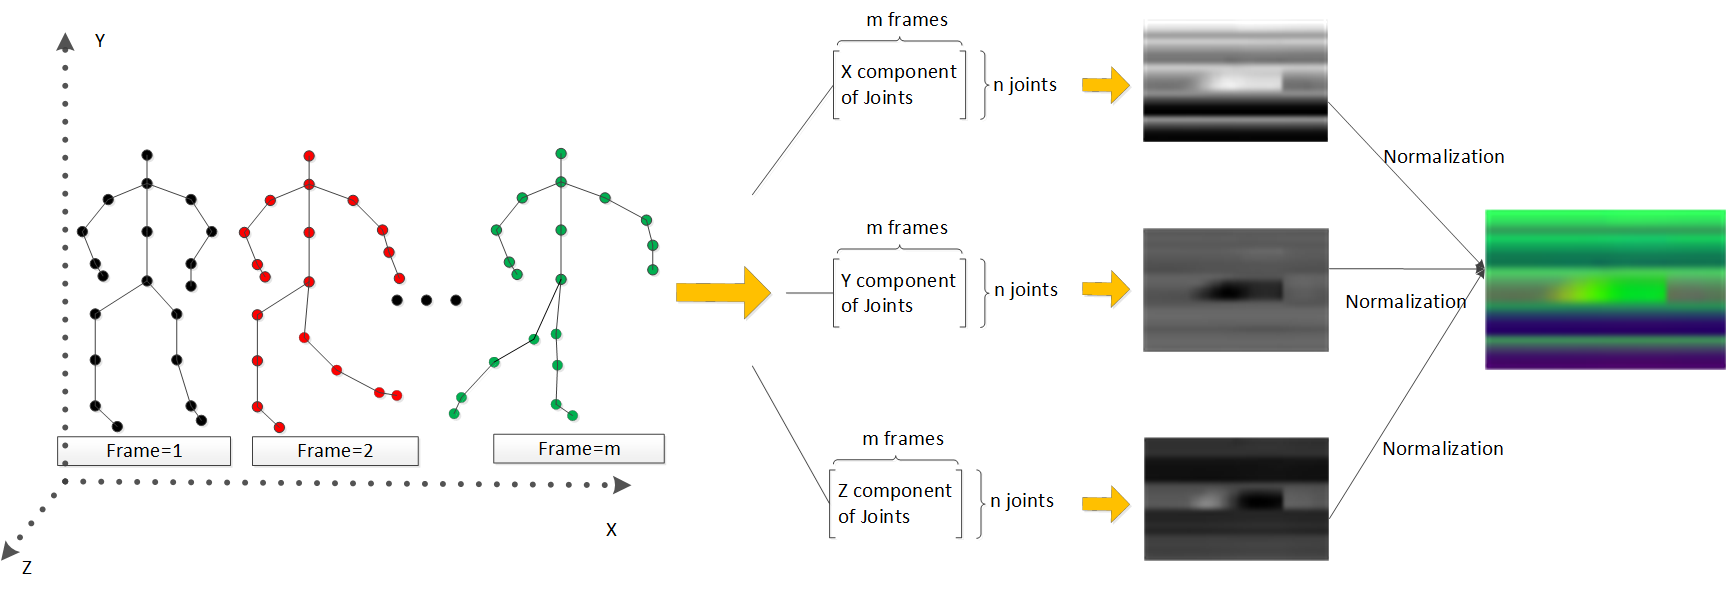
\includegraphics[scale=0.95]{images/Figure_2.png}
\caption{Each pixel represent a skeleton joint in skeleton image. Even the pixel around the corner(A,C) has equally importance to the one(B) located in the center. While things didn’t usually happen in natural image.}

\label{fig:2}
\end{figure*}

\begin{figure*}	[htb]
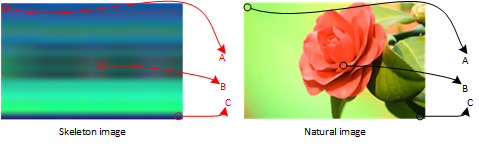
\includegraphics[scale=0.24]{images/Figure_3.png}
\caption{CNN architecture of the mapping function $F_W$: Three dilated-dense blocks are designed to enhance the robust representation of the skeleton image. The parameter W of the mapping function is corresponding to the weights and biases of the CNN network.}
\label{fig:3}
\end{figure*}

\subsection*{The Model}
Given $K$ classes of labeled skeleton image samples, we randomly subsample a few of samples from each class as the support sets. The k-th support set can be defined as:
$$S_k=I_1,I_2,\cdots I_{N_s}$$

The support sets will be mapped into a metric space by the convolution layers and the prototype of k-th class $c_k$ is the mean of the mapped support samples that belong to it . \reffig{fig:1} illustrate the structure of the action recognition model.

$$c_k=\frac{1}{N_s} \sum \limits_{I_i,y_i\in S_k}F_W (I_i)$$

When feeding an unlabeled skeleton image $I^*$, the label of the image is decided by the nearest neighbour prototype, from whom it has the shortest distance.

$$\mathop{\arg\min}_{i} \left( \lVert F_W \left( I^\ast \right) - c_i \rVert^2 \right)$$

The inference phase of our model is similar to the nearest neighbor search. 
The algorithm 1 is a brief pseudo-code of the inference phase.

\begin{figure*}	[htb]
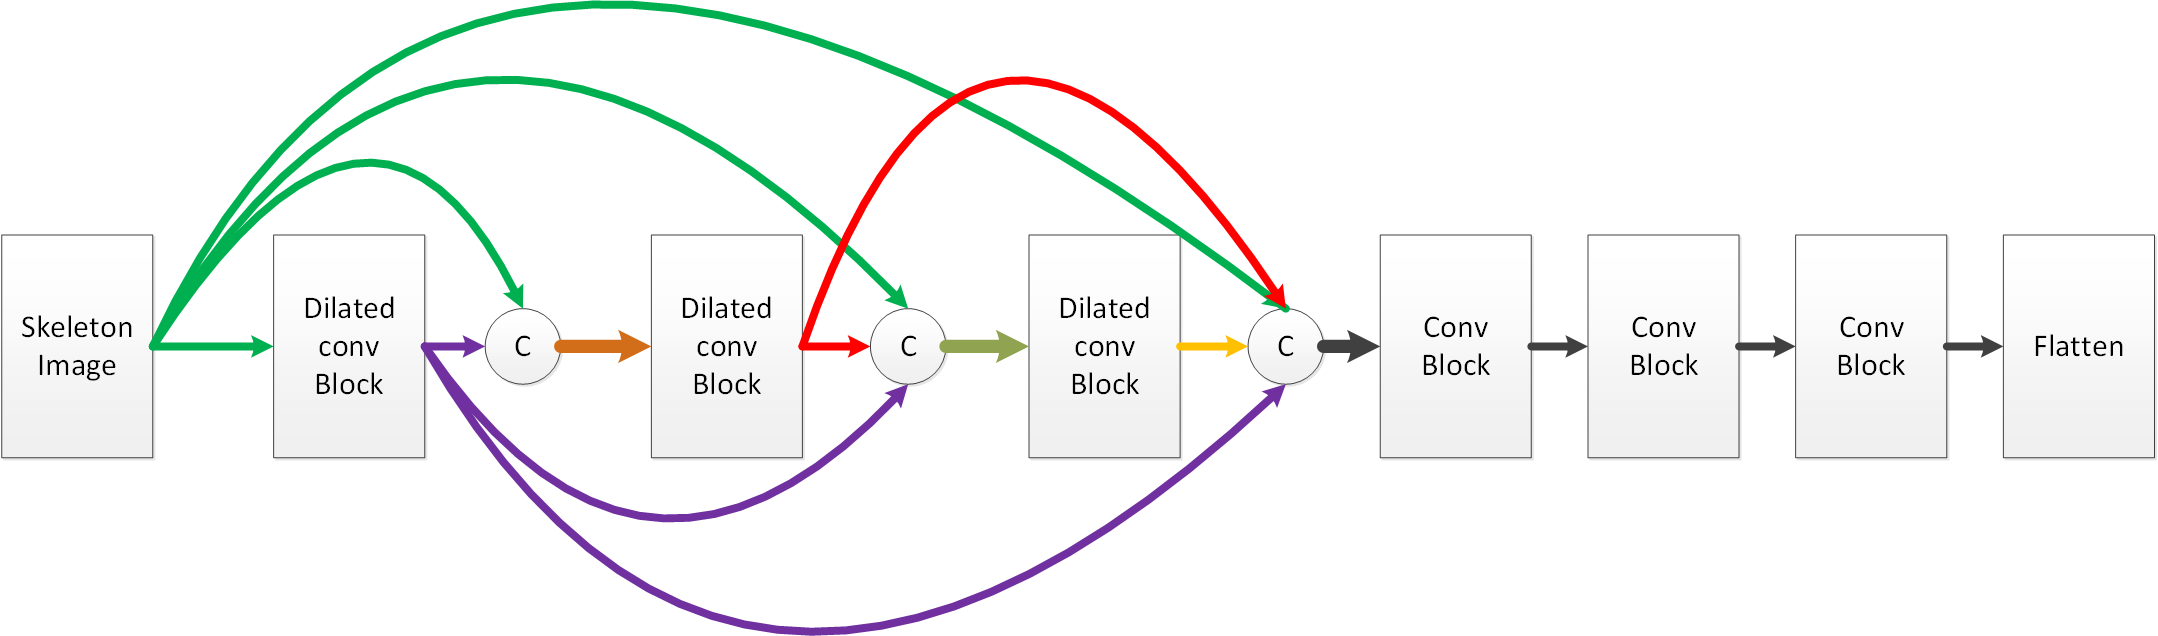
\includegraphics[width=12.93cm,height=5.33cm]{images/Figure_4.png}
\caption{The structure of the skeleton-based action recognition model. Sample $A^\ast$ is assigned to the class whose prototype had the shortest distance from it}
\label{fig:4}
\end{figure*}
\begin{algorithm}
\caption{ the inference process of action recognition model.}
\KwIn{$k$ classes of support set $S=\{S^1,S^2,\cdots S^k \}$, where each class of support}
\KwOut{the assignment of the unlabeled sample $y^*$}
\label{alg:1}
	\ForEach{\bf{i in K}}
	{
	
	$\mathbf{I^i}=\{I^i_1,I^i_2,\cdots I^i_N\}=\mathbf{Encode}(S^i)$
	
	$\mathbf{F^i}=\{F^i_1,F^i_2,\cdots F^i \{ N_s \} \}=\mathbf{F_w(I^i)}$
	
	$\mathbf{c_i}\leftarrow mean(F^i)$
	
	}
	
	$I^\ast = \mathbf{Encode}(a^\ast) $
	
	$F^\ast = \mathbf{F_w}(I^\ast)$
	
	$y^\ast=\mathop{\mathbf{argmin}}\limits_{\mathbf{i}} \left( \lVert F_W \left( I^\ast \right) - c_i \rVert^2 \right)$
\end{algorithm}

The parameter of our model can be divided into two subsets. One is the support sets $C_{support}=\{c_1,c_2,\cdots c_K\}$it can be provided by a few labeled samples in real recognition scenarios. The other one is the parameter of the mapping function $F_W$, which can be solved via SGD optimization. The purpose of our training algorithm is to address the learnable parameter of w. The training samples are divided into support and query sets. Support sets are used to estimate the prototype of each classes. While the query sets will be mapped into metric space to adjust the learnable parameter of $F_W$. For each labeled query sample $(I^\ast,y^\ast)$, The cross-entropy loss of the prototypical model can be defined as:

$$loss( y^\ast | I^\ast,C_{support},W)=\log(\frac{\exp (-d(F_W(I^\ast),c_{y^\ast}))}{\sum_{i=1}^{k}\exp((F_W(I^\ast),c_i)})$$

\reffig{fig:5} illustrates the detail computation of the cross-entropy loss of the model. Having the loss function defined, the parameters can be updated via the gradient descent method on it. We optimize the parameters of the model in few shot fashion[]. For each training iteration, we randomly divided the training samples into the support and query set. With which the cross-entropy loss of the model will be calculated. A detail description of training phase is provided in algorithm 
2.
\begin{figure*}[htb]
\centering
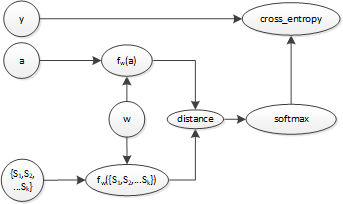
\includegraphics{images/Figure_5.png}
\caption{The computational graph of the model.}
\label{fig:5}
\end{figure*}

\begin{algorithm}
	\caption{ the training process of action recognition model.}
	\KwIn{$k$ classes of action training set $A=\{A^1,A^2,\cdots A^k\}$, where the i-th class of training sample $A^i=\{a_1^i,a_2^i,\cdots a_N^i\}$ is labeled as $y^i$ and contains $N=N_s+N_q$ samples. $N_s$ and $N_q$ are the number of support and query sample.}
	\KwOut{$W$}
	\label{alg:2}
	\bf{Init $W$}
	
	\ForEach{\bf{i in K}}
	{
		$\mathbf{I^i}=\{I^i_1,I^i_2,\cdots I^i_N\}=\mathbf{Encode}(S^i)$
		
		$\mathbf{F^i}=\{F^i_1,F^i_2,\cdots F^i \{ N_s \} \}=\mathbf{F_w(I^i)}$
	}	
			
	\Repeat{}
	{
		\ForEach{\bf{i in K}}
		{
			$F^i_{supprot}\leftarrow RandomSample(F^i,N_s)$
			
			$F^i_{query}\leftarrow F^i\-- F^i_{support}$
			
			$c_i\leftarrow mean(F^i_{support})$
		}
		$C_{support}\leftarrow \{c_1,c_2,\cdots c_k\}$
		
		$J\leftarrow0$
		
		\ForEach{\bf{i in K}}
		{
			\ForEach{\bf{$F_{it}$ in $F^i_{query}$}}
			{
				
				$J\leftarrow J+ \frac{1}{N_q*K}log\{p(y^i|F_it,C_{support},W)\}$
			}	
		}
		$W^{new}\leftarrow W^{old}\-- \epsilon\bigtriangledown_W J$
	}
	
	$I^\ast = \mathbf{Encode}(a^\ast) $
	
	$F^\ast = \mathbf{F_w}(I^\ast)$
	
	$y^\ast=\mathop{\mathbf{argmin}}\limits_{\mathbf{i}} \left( \lVert F_W \left( I^\ast \right) - c_i \rVert^2 \right)$
\end{algorithm}

%-------------------------------------------------------------------------
\section{Experiments}
The whole architecture of our model is provide in \reffig{fig:4}, as mentioned before, we construction the mapping function as a serial of dilated-dense layers. The structure of network is illustrated in \reffig{fig:3}. It composed of three dilated-dense blocks, three convolution blocks and a flatten layer. We implemented our method on Tensorflow with GTX 1080 and evaluated it on two popular benchmarks. Our model requires less training examples than existing algorithm with a comparable accuracy. A reproducible piece of code is available in
 \url{https://github.com/NanYoMy/human_action_recognition}

\subsection*{UTD-MHAD}
The UTD-MHAD dataset contains 27 classes of actions performed by 8 subjects (4 females and 4 males), Each subject repeated each action 4 times[20]. So, we get 32 samples per action. From each type of action, we select 8 sequences as the training set, and leave out 24 samples for testing. For evaluation, we randomly generated 4 support samples per class from the training set to estimate the prototypes of the model. \reftab{tab:1} shows the recognition accuracy of different methods on UTD-MHAD dataset. Compare to other algorithm, our method only needs a quarter of samples for training without any data augmentation mechanism [2,21], but still, we obtain an improvement of 1\% over the state-of-the-art .


\begin{table}[htb]
	\begin{center}
		\caption{ comparison of different action recognition methods on UTD-MHAD.}
		\begin{tabular}{|c|c|}
			\hline
			Method & Accuracy \\
			\hline
			ELC-KSVD & 76.19\% \\
			\hline
			kinect \& Inertial & 79.10\% \\
			\hline
			Cov3DJ & 85.58\%\\
			\hline
			SOS & 86.97\% \\
			\hline
			JTM & 96.27\% \\
			\hline
			TSIIM-MSDCNN[21] & 86.97\% \\
			\hline
			Our Model & \bf{97.62\%} \\
			\hline
		\end{tabular}	
	\end{center}	
	\label{tab:1}
\end{table}

\subsection*{KARD}

The KARD[22] dataset contains 18 actions, performed by 10 subjects and each subject repeated each action 3 times for creating a number of 540 sequences. Following the evaluation protocol in [2], the whole dataset is divided into three subsets. For each subset, one-third samples is used for training and the rest is for testing. Furthermore, we also train our model on the whole KARD dataset. Although the output class number is increased to 18, the model still achieves 99.38\% recognition accuracy.

\begin{table}[htb]
	\begin{center}
		\caption{ comparison of different action recognition methods on KARD. }
		\scalebox{1.1}
		{
		\begin{tabular}{|c|c|c|c|}
			\hline
			Method & Exp1 & Exp2 & Exp3 \\
			\hline
			Gaglio et al. & 89.73\% & 94.50\%&88.27\%\\
			\hline
			Cippitelli et al.; P = 11 & 96.47\% & 98.27\% & 96.87\%\\
			\hline
			Ling et al. & 98.90\% & 99.60\% & 99.43\%\\
			\hline
			DRNN[2] & 99.87\% & 98.27\% & 96.87\%\\
			\hline
			\textbf{Our Model} & \textbf{99.37\%} & \textbf{99.72\%} & \textbf{99.37\%} \\
			\hline
			\textbf{Our Model} &  \multicolumn{3}{|c|}{\textbf{99.38\%}}\\
			\hline
		\end{tabular}
		}
	\end{center}
	
	\label{tab:2}
\end{table}

\subsection*{Few (one) shot action recognition}
To investigate the performance of the model when dealing with the samples from the unseen class, we must evaluate it with the action that have not presented during the training phase. For this purpose, the all class of the dataset is split into two disjoint sets as showed in \reftab{tab:3}. Parameter of the mapping function is optimized on training set. For evaluation , we randomly select few(one) support samples per class from the testing set to estimate the prototypes of the model. And the rest testing samples are used to validate the accuracy. \reftab{tab:4} gives the performance of the model on the unseen action without retraining the parameter of the mapping function. 
\begin{table}[htbp]
	\begin{center}
		\caption{ list of action in two disjoint sets (training set and testing set). }
		
		\begin{tabular}{|c|p{4.8cm}|p{4cm}|}
	
			\hline
			  & Training Set & Testing Set  \\
			\hline
			UTD-MHAD & (1) right arm swipe to the left, (2) right arm swipe to the right, (3) right hand wave, (4) two hand front clap, (5) right arm throw, (6) cross arms in the chest, (7) basketball shoot, (8) right hand draw x, (9) right hand draw circle (clockwise), (10) right hand draw circle (counter clockwise), (11) draw triangle, (12) bowling (right hand), (13) front boxing, (14) baseball swing from right, (15) tennis right hand forehand swing, (16) arm curl (two arms), (17) tennis serve & (18) two hand push, (19) right hand knock on door, (20) right hand catch an object, (21) right hand pick up and throw, (22) jogging in place, (23) walking in place, (24) sit to stand, (25) stand to sit, (26) forward lunge (left foot forward), (27) squat (two arms stretch out)\\
			\hline
			\bfseries{KARD} & 1 Horizontal arm wave, 2 High arm wave
			3 Two hand wave, 4 Catch Cap, 5 High throw, 6 Draw X, 7 Draw Tick, 8 Toss Paper, 9 Forward Kick, 10 Side Kick
			 & 1 Take Umbrella, 12 Bend, 13 Hand Clap, 14 Walk, 15 Phone Call, 16 Drink, 17 Sit down, 18 Stand up \\
			\hline
		\end{tabular}	
	\end{center}	
	\label{tab:3}
\end{table}


\begin{table*}[htbp]
	\begin{center}
		\caption{ the classification accuracies of the model with different number of support samples on UTD-MHAD and KARD datasets. All accuracy result is averaged over 1000 test episodes. }
		
		\begin{tabular}{|c|c|c|}
			
			\hline
			& UTD-MHAD & KARD\\
			\hline
			5 support samples & (1) 93.5\% & 95.88\% \\
			\hline
			1 support samples & 82.54\%
			& 87.3\%\\
			\hline
		\end{tabular}	
	\end{center}	
	\label{tab:4}
\end{table*}
%-------------------------------------------------------------------------
\section{Conclusion}

We present an action recognition method based on a few shot learning. It is able to achieve a comparable performance even with a few training samples. And we also demonstrate that our method can classify the unseen actions without retrain the parameter of the model. But, the ability of the model is limited, our method cannot be applied to the long-term skeleton sequence, which may contain a different type of continue actions. In the future, we will extend our action recognition task to the segmentation of the long-term skeleton sequence based on the few shot learning.


%------------------------------------------------------------------------
\section{Acknowledgment}
This work was supported in part by the Educational research projects for young and middle-aged teachers of Fujian under Grants 

\bibliography{egbib}

\end{document}
